\documentclass[a4paper]{scrartcl}

\usepackage[utf8]{inputenc}
\usepackage{tikz}
    \usetikzlibrary{arrows.meta, decorations.pathmorphing, backgrounds, positioning, fit, petri}
    \usetikzlibrary{positioning}

\begin{document}

\section{Polar coordinates}

Specify the angle and the distance, separated by a colon as in (30 : 1cm). Muito útil para desenhar diagramas fasoriais.

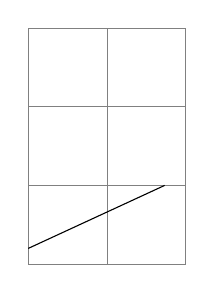
\begin{tikzpicture}
    \draw[help lines] (0,0) grid (2,3);
    \draw (0cm,2mm) -- (30:2cm);
\end{tikzpicture}

\section{Diagramas fasoriais} 

\begin{tikzpicture}
    [
        help lines/.style = {
            draw=gray!50
        },
    ]
    \clip (0,0) circle [radius=3];
    \draw[help lines] (-5,-5) grid (5,5);
    \draw[->] (0,0) -- (0:2);
    \draw[->] (0,0) -- (120:2);
    \draw[->] (0,0) -- (-120:2);
\end{tikzpicture}

\begin{tikzpicture}
    [
        help lines/.style = {
            draw=gray!20, thin
        },
    ]
    \clip (0,0) circle [radius=3];
    %\draw[help lines] (-5,-5) grid (5,5);
    \draw[help lines] (0,0) -- (30:3);
    \draw[help lines] (0,0) -- (60:3);
    \draw[help lines] (0,0) -- (90:3);
    \draw[help lines] (0,0) -- (120:3);
    \draw[help lines] (0,0) -- (150:3);
    \draw[help lines] (0,0) -- (180:3);
    \draw[help lines] (0,0) -- (210:3);
    \draw[help lines] (0,0) -- (240:3);
    \draw[help lines] (0,0) -- (270:3);
    \draw[help lines] (0,0) -- (300:3);
    \draw[help lines] (0,0) -- (330:3);
    \draw[->] (0,0) -- (0:2);
    \draw[->] (0,0) -- (120:2);
    \draw[->] (0,0) -- (-120:2);
\end{tikzpicture}
    
\section{Tutorial de Nodes}

\begin{tikzpicture}
    %\usetikzlibrary{arrows.meta, decorations.pathmorphing, backgrounds, positioning, fit, petri}
    \path (0,2) node [shape=circle,draw] {}
        ( 0,1) node [shape=circle,draw] {}
        ( 0,0) node [shape=circle,draw] {}
        ( 1,1) node [shape=rectangle,draw] {}
        (-1,1) node [shape=rectangle,draw] {};
\end{tikzpicture}

\begin{tikzpicture}
    \node at ( 0,2) [circle,draw] {};
    \node at ( 0,1) [circle,draw] {};
    \node at ( 0,0) [circle,draw] {};
    \node at ( 1,1) [rectangle,draw] {};
    \node at (-1,1) [rectangle,draw] {};
\end{tikzpicture}

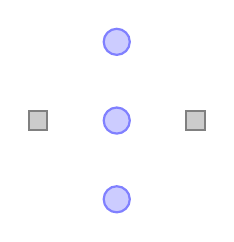
\begin{tikzpicture}
    %defining some styles
    [
        place/.style={circle, draw=blue!50, fill=blue!20, thick},
        transition/.style={rectangle, draw=black!50, fill=black!20, thick},
    ]
    \node at ( 0,2) [place] {};
    \node at ( 0,1) [place] {};
    \node at ( 0,0) [place] {};
    \node at ( 1,1) [transition] {};
    \node at (-1,1) [transition] {};
\end{tikzpicture}

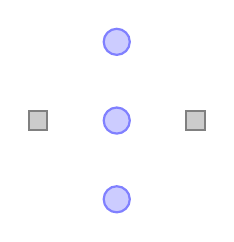
\begin{tikzpicture}
    [
        place/.style={circle, draw=blue!50, fill=blue!20, thick},
        transition/.style={rectangle, draw=black!50, fill=black!20, thick},
    ]
    \node (waiting) at (0,2) [place] {};
    \node (critical) at (0,1) [place] {};
    \node (semaphore) at (0,0) [place] {};
    \node (leave critical) at (1,1) [transition] {};
    \node (enter critical) at (-1,1) [transition] {};
\end{tikzpicture}

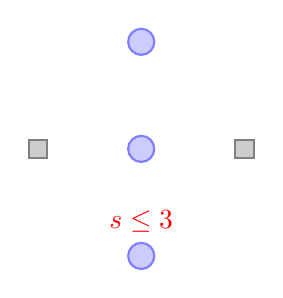
\begin{tikzpicture}
    %\usetikzlibrary{positioning}
    [
        place/.style={circle, draw=blue!50, fill=blue!20, thick},
        transition/.style={rectangle, draw=black!50, fill=black!20, thick},
    ]
    \node[place] (waiting) {};
    \node[place] (critical) [below=of waiting] {};
    \node[place] (semaphore) [below=of critical] {};
    \node[transition] (leave critical) [right=of critical] {};
    \node[transition] (enter critical) [left=of critical] {};

    \node[red,above] at (semaphore.north) {$s \le 3$};
\end{tikzpicture}

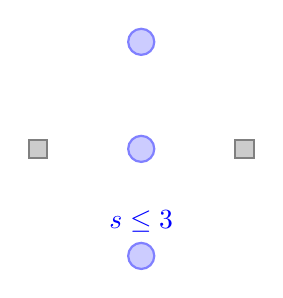
\begin{tikzpicture}
    %\usetikzlibrary{positioning}
    [
        place/.style = {
            circle, draw=blue!50, fill=blue!20, thick
            },
        transition/.style = {
            rectangle, draw=black!50, fill=black!20, thick
            },
        every label/.style = {
            blue
            },
    ]
    \node[place] (waiting) {};
    \node[place] (critical) [below=of waiting] {};
    \node[place] (semaphore) [below=of critical,
                                label=above:$s\le3$] {};
    \node[transition] (leave critical) [right=of critical] {};
    \node[transition] (enter critical) [left=of critical] {};
\end{tikzpicture}

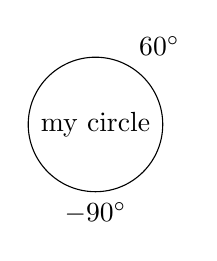
\begin{tikzpicture}
    \node[circle,
        draw,
        label=60:$60^\circ$,
        label=below:$-90^\circ$,
        ] {my circle};
\end{tikzpicture}

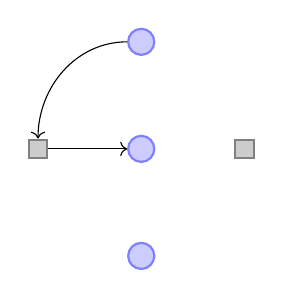
\begin{tikzpicture}
    %\usetikzlibrary{positioning}
    [
        place/.style = {
            circle, draw=blue!50, fill=blue!20, thick
            },
        transition/.style = {
            rectangle, draw=black!50, fill=black!20, thick
            },
        every label/.style = {
            blue
            },
    ]
    %nodes
    \node[place] (waiting) {};
    \node[place] (critical) [below=of waiting] {};
    \node[place] (semaphore) [below=of critical] {};
    \node[transition] (leave critical) [right=of critical] {};
    \node[transition] (enter critical) [left=of critical] {};
    %connecting nodes
    \draw [->] (enter critical.east) to (critical.west);
    \draw [->] (waiting.west) to[out=180, in=90] (enter critical.north);

\end{tikzpicture}


\end{document}

